\documentclass[conference]{IEEEtran}

% =========================
% Packages
% =========================
\usepackage[T1]{fontenc}
\usepackage[utf8]{inputenc}
\usepackage{cite}
\usepackage{amsmath,amssymb,amsfonts}
\usepackage{graphicx}
\usepackage{textcomp}
\usepackage{xcolor}
\usepackage{booktabs}
\usepackage{multirow}
\usepackage{array}
\usepackage{url}
\usepackage{hyperref}
\usepackage{balance}

% Keep double-column figures from stacking on the same page.
\setcounter{dbltopnumber}{1}
\renewcommand{\dbltopfraction}{0.85}
\renewcommand{\textfraction}{0.08}
\renewcommand{\floatpagefraction}{0.75}
\renewcommand{\dblfloatpagefraction}{0.75}

\hypersetup{
  colorlinks=true,
  linkcolor=black,
  citecolor=green!50!black,
  urlcolor=blue
}

\begin{document}

\title{From Direct Transfer to Fine-Tuning: A Cross-Dataset Study of TwinLiteNet+ for Road Scene Segmentation}

\author{
  \centering
  \small
  \begin{tabular}{>{\centering\arraybackslash}p{0.31\textwidth}
      >{\centering\arraybackslash}p{0.31\textwidth}
    >{\centering\arraybackslash}p{0.31\textwidth}}
    Thai-Thong Nguyen &
    Thanh-Hai Hoang &
    Bich-Loan Thi Le \\[-1pt]

    \textit{University of Science, VNU-HCM} &
    \textit{University of Science, VNU-HCM} &
    \textit{University of Science, VNU-HCM} \\

    Vietnam National University Ho Chi Minh City &
    Vietnam National University Ho Chi Minh City &
    Vietnam National University Ho Chi Minh City \\

    {\scriptsize 25C1106749@student.hcmus.edu.vn} &
    {\scriptsize 25C1103807@student.hcmus.edu.vn} &
    {\scriptsize 25C1202757@student.hcmus.edu.vn}
  \end{tabular}
}

\maketitle

\begin{abstract}
  This paper evaluates the cross-dataset transferability of TwinLiteNet+, a lightweight model for joint drivable area and lane segmentation. We keep the original architecture unchanged and test the official pretrained checkpoints on two target datasets, Mapillary Vistas and Cityscapes, after converting their semantic annotations into TwinLiteNet+-compatible targets. Direct transfer shows a clear degradation outside BDD100K: for the Large variant, drivable area mIoU reaches 70.4\% on Mapillary Vistas and 79.5\% on Cityscapes, while lane IoU drops to 6.5\% and 1.5\%, respectively. After fine-tuning, the same Large model improves to 77.0\% drivable area mIoU and 21.9\% lane IoU on Mapillary Vistas, and to 93.4\% drivable area mIoU on Cityscapes. The Cityscapes lane branch remains limited, reaching only 6.2\% lane IoU, because its lane target is based on an approximate proxy label. These results show that TwinLiteNet+ can adapt well to new domains when target annotations are semantically compatible, but its lane branch is highly sensitive to label mismatch.
\end{abstract}

\begin{IEEEkeywords}
  TwinLiteNet+, cross-dataset generalization, drivable area segmentation, lane segmentation, domain shift, Cityscapes, Mapillary Vistas
\end{IEEEkeywords}

\section{Introduction}
Drivable area segmentation and lane segmentation are two core perception tasks in autonomous driving. Together, they provide dense and directly actionable information for vehicle control, path planning, and scene understanding. In practical deployment, however, a model is rarely tested only on data drawn from the same distribution as the training set. Differences in geographic region, camera characteristics, weather conditions, road layout, and annotation policy can introduce domain shift, causing a model that performs well on one benchmark to degrade substantially on another.

TwinLiteNet+ was originally proposed as a lightweight multi-task network for drivable area and lane segmentation~\cite{ref1}. The architecture combines a hybrid encoder based on stride-based dilated convolutions and depthwise separable dilated convolutions, a Partial Class Activation Attention (PCAA) module, and dual task-specific decoders. It is also available in four scalable configurations---Nano, Small, Medium, and Large---to support different computational budgets. On BDD100K, TwinLiteNet+ achieved strong segmentation accuracy while maintaining low model complexity and practical suitability for real-time deployment~\cite{ref1,ref2}.

The practical question is not only whether TwinLiteNet+ performs well on its source benchmark, but also what happens when the same model is moved to a new dataset. This question is important because a road-scene model used in practice may encounter different cities, camera viewpoints, lane marking styles, and annotation rules. A lightweight model can be attractive for deployment, but its usefulness depends on whether its learned representation remains meaningful beyond the dataset used during training.

In this work, we study cross-dataset generalization rather than architectural redesign. We keep the original TwinLiteNet+ architecture unchanged and evaluate it under two transfer settings. In the first setting, we directly apply pretrained weights from the source domain to target datasets in order to measure out-of-domain generalization. In the second setting, we fine-tune the same pretrained model on each target dataset to analyze how much performance can be recovered through adaptation. Since TwinLiteNet+ was originally designed for drivable area and lane segmentation, we also define a label harmonization procedure that maps the annotations of Cityscapes and Mapillary Vistas into a task formulation compatible with the original model outputs~\cite{ref3,ref4}.

This setting differs from typical domain adaptation studies. We do not add adversarial training, image translation, self-training, or a new model component. Instead, we focus on a simpler but common situation: a practitioner has a pretrained checkpoint and wants to know whether direct evaluation is reliable, whether supervised fine-tuning is enough, and which output branch is more vulnerable to dataset and label changes. This makes the study narrower than a full adaptation method, but also easier to reproduce and interpret.

The main contributions of this work are summarized as follows:
\begin{itemize}
  \item We evaluate the cross-dataset generalization capability of the original TwinLiteNet+ on Cityscapes and Mapillary Vistas for drivable area and lane segmentation.
  \item We introduce a label harmonization procedure that converts the annotations of the target datasets into labels compatible with the original TwinLiteNet+ outputs.
  \item We compare two practical transfer settings: direct transfer using source-domain pretrained weights and target-specific fine-tuning initialized from those same weights.
  \item We quantify how much performance is lost under cross-dataset transfer and how much can be recovered through fine-tuning, with particular attention to the different behavior of the drivable area and lane branches.
\end{itemize}

\section{Related Work}

\subsection{Lightweight Road-Scene Segmentation}
Real-time road-scene segmentation is usually a compromise between spatial detail, semantic context, and inference cost. ENet is an early example of pushing this compromise toward speed by using a compact encoder-decoder design for real-time semantic segmentation~\cite{ref5}. Its strength is efficiency, but it is a general semantic segmentation network and does not model drivable area and lane prediction as two related outputs. BiSeNet addresses another part of the same trade-off by separating a spatial path from a context path, while BiSeNet V2 refines this idea with a detail branch and a semantic branch connected through guided aggregation~\cite{ref6,ref7}. These models are useful references because they show how lightweight segmentation networks preserve boundary information without relying on heavy backbones.

TwinLiteNet+ is closer to the target application of this paper than the above general semantic segmentation models. It is built specifically for joint drivable area and lane segmentation, with a shared encoder, a PCAA module, and two task-specific decoders~\cite{ref1}. Its Nano-to-Large variants also make it convenient to compare different model capacities under one architecture. What the original study does not emphasize, however, is how the same dual-branch model behaves when its test data and label definitions move away from BDD100K~\cite{ref1,ref2}. That gap motivates our evaluation.

\subsection{Domain Shift and Adaptation for Segmentation}
Domain shift in semantic segmentation has been studied mostly through adaptation methods. Output-space adaptation aligns structured predictions between source and target domains, assuming that segmentation outputs carry useful spatial regularities across domains~\cite{ref8}. CyCADA adds another route by combining image-level translation with feature-level alignment, reducing both appearance and representation gaps~\cite{ref9}. DAFormer later shows that architecture and training strategy can strongly affect adaptation quality on road-scene benchmarks~\cite{ref10}.

These works are important, but their problem setting is different from ours. They usually aim to design an adaptation algorithm, often with a source and target label space that is already compatible. Our case is more restricted and more practical: we do not add an adversarial loss, image translation, or self-training stage. Instead, we ask how far an existing lightweight model can go with two common choices available to a practitioner: direct evaluation of a pretrained checkpoint and supervised fine-tuning after converting the target labels into the original task format.

\subsection{Road-Scene Benchmarks and Label Alignment}
BDD100K, Cityscapes, and Mapillary Vistas are all road-scene datasets, but they are not interchangeable. BDD100K is the source benchmark used by TwinLiteNet+ and supports driving-related tasks including drivable area and lane segmentation~\cite{ref1,ref2}. Cityscapes provides high-quality semantic labels for structured urban scenes, but it does not provide a lane-marking class that directly matches the TwinLiteNet+ lane branch~\cite{ref3}. Mapillary Vistas covers more diverse scenes and has a richer semantic label set, which gives more room to build lane-related targets, although the mapping is still not identical to BDD100K~\cite{ref4}.

This annotation mismatch is not a minor implementation detail. It directly affects what the model is asked to predict after transfer. A high drivable-area score can still be meaningful on Cityscapes because the road class is well aligned with the target branch, whereas the lane branch becomes less reliable when the only available proxy is the ground class. For this reason, our experiments treat label construction as part of the evaluation design rather than as a preprocessing footnote.

\subsection{Position of This Study}
The paper is placed between two lines of work. From lightweight segmentation, it inherits the concern for compact multi-task road perception~\cite{ref1,ref5,ref6,ref7}. From domain-shift studies, it takes the question of whether a model learned on one domain remains useful on another~\cite{ref8,ref9,ref10}. The difference is that we keep the model and adaptation method deliberately simple. The focus is not to outperform domain adaptation methods, but to measure what happens to TwinLiteNet+ when the dataset changes and the labels have to be reconstructed for its two output branches.

\section{Methodology}
We evaluate TwinLiteNet+ in a controlled transfer setting. The network itself is not changed; the dataset-specific components are the label construction rules and the fine-tuning data. This separation keeps the experiment centered on two sources of performance change: visual domain shift and annotation mismatch.

\subsection{Base Architecture}
TwinLiteNet+ is used in the same form as the original implementation~\cite{ref1}. The model contains a shared encoder, the PCAA module, and two decoders, one for drivable area segmentation and one for lane segmentation. We keep the four released variants---Nano, Small, Medium, and Large---so that the effect of model scale can be observed without introducing another architecture.

In our setting, the two branches are important because they do not transfer equally. Drivable area segmentation is usually tied to large road regions, while lane segmentation depends on thinner structures and more specific annotations. Keeping the original branches therefore lets us see which part of the learned representation is more robust under a new dataset. Fig.~\ref{fig:twinlitenet_arch} shows the architecture used in the experiments.

\begin{figure*}[!t]
  \centering
  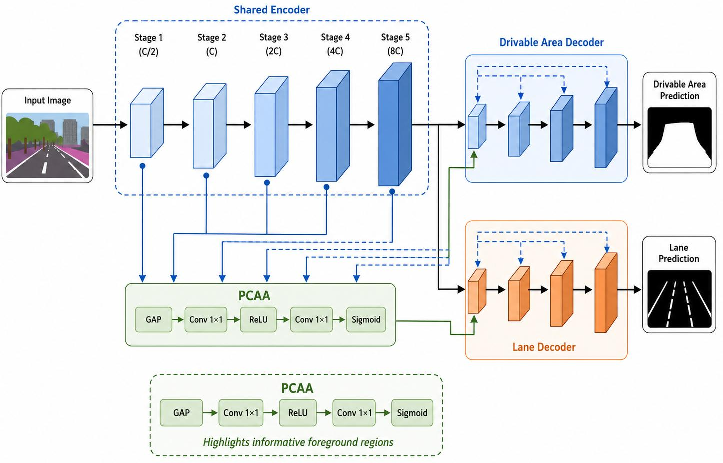
\includegraphics[width=0.78\textwidth]{figs/twinlitenet_architecture_final.pdf}
  \caption{Overall architecture of TwinLiteNet+. The original shared encoder, PCAA module, and two task-specific decoders are kept unchanged. The figure is intentionally simplified so that the caption explains the role of the architecture rather than repeating implementation details inside the diagram.}
  \label{fig:twinlitenet_arch}
\end{figure*}

\subsection{Target Label Construction}
Cityscapes and Mapillary Vistas cannot be used directly with TwinLiteNet+ because their annotations are semantic segmentation labels rather than the original BDD100K drivable-area and lane labels~\cite{ref3,ref4}. We therefore convert each target dataset into two binary target groups: drivable area and lane-related regions. The mapping is intentionally simple and reproducible; it is not meant to claim that the converted labels are perfectly equivalent to BDD100K.

For Mapillary Vistas, the drivable area target is formed by merging road-related classes, including \textit{road}, \textit{service-lane}, \textit{driveway}, \textit{parking}, \textit{parking-aisle}, \textit{road-shoulder}, and \textit{bike-lane}. The lane target is built from lane-marking and crosswalk-related classes. Since Mapillary Vistas contains more fine-grained road-scene labels than BDD100K~\cite{ref2,ref4}, its converted lane branch is imperfect but still informative.

For Cityscapes, the mapping is more limited. The \textit{road} class is used for the drivable area branch, which is a reasonable semantic match. The lane branch has no direct counterpart, so we use \textit{ground} only as a proxy. This makes the Cityscapes lane results useful for observing transfer behavior, but not for claiming strict lane-marking performance.

Table~\ref{tab:dataset_summary} summarizes the construction rules, and Fig.~\ref{fig:label_harmonization} gives a compact visual overview of the mapping process.

\begin{figure*}[!t]
  \centering
  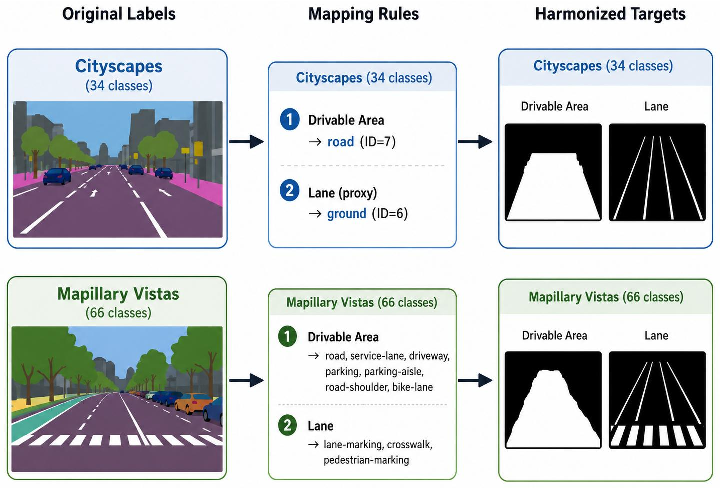
\includegraphics[width=0.76\textwidth]{figs/label_harmonization_final.pdf}
  \caption{Label harmonization process for Cityscapes and Mapillary Vistas. The target datasets provide semantic segmentation labels, so their annotations are converted into the two branches required by TwinLiteNet+: drivable area and lane-related regions. The Cityscapes lane branch is based on a proxy label, while Mapillary Vistas provides richer road-marking information.}
  \label{fig:label_harmonization}
\end{figure*}

\subsection{Transfer Protocol}
We use two transfer settings. The first is \textit{direct transfer}: the pretrained TwinLiteNet+ checkpoints are evaluated on the target datasets without further optimization. This is the stricter test because the model must rely only on what it learned from the source domain.

The second setting is \textit{target-specific fine-tuning}. Starting from the same pretrained checkpoint, the model is trained again on the target dataset using the constructed labels. Architecture and loss design remain unchanged, so the observed gain mainly reflects how much target supervision helps the original model adapt.

The workflow is summarized in Fig.~\ref{fig:experimental_protocol}. BDD100K is treated as the source domain, while Cityscapes and Mapillary Vistas are the two target domains~\cite{ref2,ref3,ref4}.


\section{Experiments}

\subsection{Experimental Setup}
The experiments follow the transfer protocol above. We first re-validate the official checkpoints on BDD100K to check that our evaluation code matches the original setting. We then run the same checkpoints on Cityscapes and Mapillary Vistas without training. Finally, we fine-tune each variant on the corresponding target dataset and evaluate again.

All four TwinLiteNet+ variants are tested: Nano, Small, Medium, and Large. Table~\ref{tab:dataset_summary} lists the dataset roles and the target-label construction used in the experiments.

\begin{table}[!t]
  \centering
  \caption{Datasets and target-label construction used in this study.}
  \label{tab:dataset_summary}
  \resizebox{\linewidth}{!}{
    \begin{tabular}{llll}
      \toprule
      Role & Dataset & Split Used & Target Construction \\
      \midrule
      Source & BDD100K & Official pretrained setting & Original DA/LL labels \\
      Target & Mapillary Vistas & 18,000 / 2,000 / 5,000 & Merged road and lane-related classes \\
      Target & Cityscapes & 2,975 / 500 / 1,525 & \textit{road} for DA, \textit{ground} proxy for lane \\
      \bottomrule
    \end{tabular}
  }
\end{table}

BDD100K is the source domain because it is the dataset used by the original TwinLiteNet+ checkpoints~\cite{ref1,ref2}. Cityscapes and Mapillary Vistas are used as target domains because they differ from BDD100K in both appearance and labeling policy~\cite{ref3,ref4}.




\subsection{Evaluation Metrics}
Following the original TwinLiteNet+ setting~\cite{ref1}, we evaluate the two output branches separately. For drivable area segmentation, we use mean Intersection over Union (mIoU). For lane segmentation, we report both lane accuracy and lane IoU.

For each class $c$, the Intersection over Union is defined as
\begin{equation}
  \mathrm{IoU}_c = \frac{TP_c}{TP_c + FP_c + FN_c},
\end{equation}
where $TP_c$, $FP_c$, and $FN_c$ denote the numbers of true positive, false positive, and false negative pixels for class $c$, respectively.

The mean Intersection over Union is computed as
\begin{equation}
  \mathrm{mIoU} = \frac{1}{C}\sum_{c=1}^{C}\mathrm{IoU}_c,
\end{equation}
where $C$ is the number of classes.

For the lane branch, pixel accuracy is computed as
\begin{equation}
  \mathrm{Accuracy} = \frac{TP + TN}{TP + TN + FP + FN},
\end{equation}
where $TP$, $TN$, $FP$, and $FN$ denote the numbers of true positive, true negative, false positive, and false negative pixels, respectively.

Lane IoU is computed as
\begin{equation}
  \mathrm{Lane\ IoU} = \frac{TP}{TP + FP + FN}.
\end{equation}

In the transfer analysis, IoU-based metrics are more informative than accuracy because lane pixels occupy only a small part of each image. We still report lane accuracy for consistency with the original evaluation.

\subsection{Implementation Details}
The implementation follows the original TwinLiteNet+ repository as closely as possible~\cite{ref1}. The model architecture and two-branch loss design are kept unchanged. The loss combines Tversky loss and focal loss as in the original implementation~\cite{ref1,ref12,ref13}. Table~\ref{tab:train_config} summarizes the main training configuration.

\begin{table}[!t]
  \centering
  \caption{Training configuration used in this study.}
  \label{tab:train_config}
  \resizebox{\linewidth}{!}{
    \begin{tabular}{ll}
      \toprule
      Parameter & Value \\
      \midrule
      Optimizer & AdamW~\cite{ref11} \\
      Initial learning rate & $5 \times 10^{-4}$ \\
      AdamW $\beta_1$ & 0.9 \\
      Weight decay & $5 \times 10^{-4}$ \\
      Learning-rate scheduler & Poly \\
      Fine-tuning epochs & 40 \\
      Input size & $384 \times 640$ \\
      Mask size & $360 \times 640$ \\
      Output crop & 12 px top, 12 px bottom \\
      Source-domain GPU & RTX A500 \\
      Target-domain GPU & Kaggle T4 \\
      \bottomrule
    \end{tabular}
  }
\end{table}

The overall training objective can be written in a general form as
\begin{equation}
  \mathcal{L}_{total} = \lambda_{da}\mathcal{L}_{da} + \lambda_{lane}\mathcal{L}_{lane},
\end{equation}
where $\mathcal{L}_{da}$ and $\mathcal{L}_{lane}$ denote the losses for the drivable area branch and the lane branch, respectively.

The polynomial learning-rate schedule is expressed as
\begin{equation}
  lr_t = lr_0\left(1 - \frac{t}{T}\right)^{p},
\end{equation}
where $lr_0$ is the initial learning rate, $t$ is the current training step, $T$ is the total number of training steps, and $p$ is the polynomial decay factor.

For preprocessing, input images are letterboxed from $720 \times 1280$ to $384 \times 640$, while the corresponding masks are resized to $360 \times 640$. Following the original implementation~\cite{ref1}, the model outputs are cropped by 12 pixels at the top and 12 pixels at the bottom before loss and metric computation. For Mapillary Vistas, the original preprocessing and augmentation strategy is retained, while for Cityscapes we use the harmonized labels without additional augmentation.

\begin{figure}[!t]
  \centering
  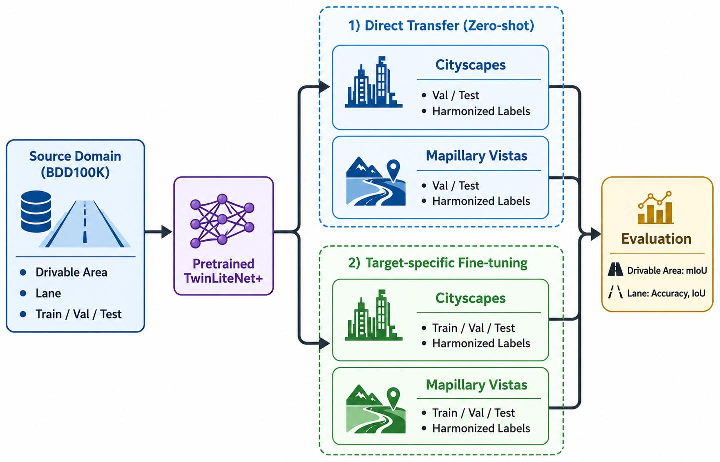
\includegraphics[width=0.88\linewidth]{figs/cross_dataset_protocol_column.pdf}
  \caption{Cross-dataset transfer protocol. The same pretrained checkpoint is evaluated directly and then fine-tuned on each target dataset. Both settings are evaluated with drivable area mIoU, lane accuracy, and lane IoU.}
  \label{fig:experimental_protocol}
\end{figure}

\subsection{Source-Domain Re-Validation}
Before moving to cross-dataset evaluation, we first re-validate the official TwinLiteNet+ checkpoints on the source-domain benchmark, BDD100K. This step verifies that our evaluation pipeline is consistent with the original repository before testing the model under domain shift.

Table~\ref{tab:bdd_reval} compares the results reported in the original paper~\cite{ref1} with the results reproduced by our group. The two sets of numbers are nearly identical across all model variants, with a maximum difference of only 0.1 percentage point. This gives us a stable baseline for interpreting the target-domain results.

\begin{table}[!t]
\centering
\caption{Source-domain re-validation on BDD100K.}
\label{tab:bdd_reval}
\resizebox{\linewidth}{!}{
\begin{tabular}{lcccccc}
\toprule
\multirow{2}{*}{Variant} & \multicolumn{3}{c}{Paper} & \multicolumn{3}{c}{Our Re-validation} \\
\cmidrule(lr){2-4} \cmidrule(lr){5-7}
& DA mIoU & Lane Acc. & Lane IoU & DA mIoU & Lane Acc. & Lane IoU \\
\midrule
Nano   & 87.3 & 70.2 & 23.3 & 87.4 & 70.2 & 23.4 \\
Small  & 90.6 & 75.8 & 29.3 & 90.6 & 75.8 & 29.3 \\
Medium & 92.0 & 79.1 & 32.3 & 92.0 & 79.1 & 32.4 \\
Large  & 92.9 & 81.9 & 34.2 & 92.9 & 81.9 & 34.2 \\
\bottomrule
\end{tabular}}
\end{table}

\subsection{Direct Transfer Results}
We next evaluate the pretrained TwinLiteNet+ models directly on the two target datasets without additional training. This stage measures the out-of-domain generalization ability of the original model.

\subsubsection{Mapillary Vistas}
Table~\ref{tab:mapillary_direct} presents the direct-transfer results on Mapillary Vistas. Compared with the BDD100K re-validation results, the performance drops substantially, especially in the lane branch. The best drivable area result is 70.4 mIoU for the Large variant, while lane IoU remains low and reaches only 6.5.

\begin{table}[!t]
\centering
\caption{Direct transfer results on Mapillary Vistas.}
\label{tab:mapillary_direct}
\resizebox{\linewidth}{!}{
\begin{tabular}{lccc}
\toprule
Variant & DA mIoU (\%) & Lane Acc. (\%) & Lane IoU (\%) \\
\midrule
Nano   & 69.7 & 52.9 & 4.9 \\
Small  & 69.7 & 53.3 & 5.5 \\
Medium & 70.3 & 53.6 & 5.9 \\
Large  & 70.4 & 54.2 & 6.5 \\
\bottomrule
\end{tabular}}
\end{table}

This behavior is expected. Mapillary Vistas differs from BDD100K not only in visual appearance, but also in the way its semantic annotations must be remapped into the drivable area and lane-related targets used by TwinLiteNet+~\cite{ref2,ref4}. The lane branch is affected more strongly because its supervision is derived from multiple original classes and is therefore less consistent than the original BDD100K lane annotations.

\subsubsection{Cityscapes}
Table~\ref{tab:cityscapes_direct} reports the direct-transfer results on Cityscapes. The drivable area branch remains at a usable level, with the Nano variant reaching 81.1 mIoU. In contrast, the lane branch almost completely fails to transfer, with lane IoU remaining between 0.9 and 1.5 across all variants.

\begin{table}[!t]
\centering
\caption{Direct transfer results on Cityscapes.}
\label{tab:cityscapes_direct}
\resizebox{\linewidth}{!}{
\begin{tabular}{lccc}
\toprule
Variant & DA mIoU (\%) & Lane Acc. (\%) & Lane IoU (\%) \\
\midrule
Nano   & 81.1 & 51.4 & 0.9 \\
Small  & 79.7 & 51.5 & 1.0 \\
Medium & 79.6 & 52.1 & 1.2 \\
Large  & 79.5 & 52.6 & 1.5 \\
\bottomrule
\end{tabular}}
\end{table}

This result is largely explained by the label definition of Cityscapes~\cite{ref3}. While the \textit{road} class can serve as a reasonable target for drivable area segmentation, the lane branch only uses the \textit{ground} class as a proxy. Therefore, the lane results in this setting should be interpreted as reference values rather than as a strict lane-segmentation benchmark.

\subsection{Fine-Tuning Results}
After evaluating direct transfer, we fine-tune the same pretrained checkpoints on each target dataset. This stage shows how much of the lost performance can be recovered once target-domain supervision is provided.

\subsubsection{Mapillary Vistas}
Table~\ref{tab:mapillary_ft} shows the fine-tuning results on Mapillary Vistas. Clear improvements are observed across all model variants. The Large model reaches 77.0 mIoU on drivable area, 63.2 lane accuracy, and 21.9 lane IoU.

\begin{table}[!t]
\centering
\caption{Fine-tuning results on Mapillary Vistas.}
\label{tab:mapillary_ft}
\resizebox{\linewidth}{!}{
\begin{tabular}{lccc}
\toprule
Variant & DA mIoU (\%) & Lane Acc. (\%) & Lane IoU (\%) \\
\midrule
Nano   & 73.4 & 58.8 & 15.1 \\
Small  & 74.7 & 60.0 & 17.2 \\
Medium & 76.3 & 61.9 & 20.0 \\
Large  & 77.0 & 63.2 & 21.9 \\
\bottomrule
\end{tabular}}
\end{table}

The gain over direct transfer is especially visible in the lane branch. For the Large variant, drivable area mIoU increases from 70.4 to 77.0, while lane IoU increases from 6.5 to 21.9. This suggests that the pretrained representation of TwinLiteNet+ remains transferable, but target-specific supervision is necessary to adapt the model to the richer semantic structure of Mapillary Vistas.

\subsubsection{Cityscapes}
Table~\ref{tab:cityscapes_ft} reports the fine-tuning results on Cityscapes. Here, the strongest improvement appears in the drivable area branch. The Large variant increases from 79.5 to 93.4 mIoU after fine-tuning.

\begin{table}[!t]
\centering
\caption{Fine-tuning results on Cityscapes.}
\label{tab:cityscapes_ft}
\resizebox{\linewidth}{!}{
\begin{tabular}{lccc}
\toprule
Variant & DA mIoU (\%) & Lane Acc. (\%) & Lane IoU (\%) \\
\midrule
Nano   & 88.6 & 51.2 & 1.9 \\
Small  & 91.0 & 50.7 & 1.8 \\
Medium & 92.3 & 51.2 & 1.7 \\
Large  & 93.4 & 53.1 & 6.2 \\
\bottomrule
\end{tabular}}
\end{table}

In contrast, the lane branch improves only modestly for most variants, and only the Large model reaches a somewhat higher lane IoU of 6.2. This is consistent with the limited label quality available for the lane branch in Cityscapes, where the supervision is derived only from the \textit{ground} class.

\subsection{Transfer Gain Summary}
Table~\ref{tab:large_gain} summarizes the direct-transfer and fine-tuning changes for the Large variant. The two datasets improve in different ways. On Mapillary Vistas, the larger gain appears in the lane branch, which increases by 15.4 points in lane IoU. On Cityscapes, the main recovery happens in drivable area segmentation, where mIoU increases by 13.9 points. This contrast supports the main interpretation of the paper: fine-tuning helps, but it helps the branch whose target labels remain semantically meaningful.

\begin{table}[!t]
\centering
\caption{Fine-tuning gains for the Large variant.}
\label{tab:large_gain}
\resizebox{\linewidth}{!}{
\begin{tabular}{lcccccc}
\toprule
\multirow{2}{*}{Dataset} & \multicolumn{3}{c}{DA mIoU (\%)} & \multicolumn{3}{c}{Lane IoU (\%)} \\
\cmidrule(lr){2-4} \cmidrule(lr){5-7}
& Direct & Fine-tuned & Gain & Direct & Fine-tuned & Gain \\
\midrule
Mapillary Vistas & 70.4 & 77.0 & +6.6 & 6.5 & 21.9 & +15.4 \\
Cityscapes       & 79.5 & 93.4 & +13.9 & 1.5 & 6.2 & +4.7 \\
\bottomrule
\end{tabular}}
\end{table}

\subsection{Comparison with Prior Work}
The purpose of this study is different from prior lightweight segmentation and domain adaptation papers. ENet, BiSeNet, and BiSeNet V2 mainly study how to design efficient segmentation architectures~\cite{ref5,ref6,ref7}. Output-space adaptation, CyCADA, and DAFormer study how to reduce domain shift by adding adaptation mechanisms or changing the training strategy~\cite{ref8,ref9,ref10}. Our experiments instead keep both the model architecture and the adaptation strategy simple. The emphasis is on measuring how much a pretrained lightweight dual-branch model can transfer when the target labels are not naturally aligned with the source task.

This comparison is important because a high-performing architecture on its original benchmark does not directly answer whether it can be reused on another dataset. TwinLiteNet+ already demonstrates a strong accuracy-efficiency trade-off on BDD100K~\cite{ref1}. Our results add a complementary view: the model can recover strong drivable area performance through fine-tuning, but its lane branch depends heavily on the quality of the target label mapping. This limitation is not visible from in-dataset evaluation alone.


\begin{table*}[!t]
\centering
\caption{Conceptual comparison with representative prior work.}
\label{tab:prior_comparison}
\resizebox{0.95\textwidth}{!}{
\begin{tabular}{llll}
\toprule
Work & Main Focus & What It Optimizes & Relation to This Study \\
\midrule
ENet~\cite{ref5} & Real-time semantic segmentation & Compact architecture and speed & General segmentation, not dual-branch road tasks \\
BiSeNet / BiSeNet V2~\cite{ref6,ref7} & Real-time urban-scene segmentation & Detail-context balance & Architecture-oriented, not cross-dataset label mismatch \\
Output-space adaptation~\cite{ref8} & Domain-adaptive segmentation & Structured output alignment & Adds adaptation objective; assumes compatible target formulation \\
CyCADA~\cite{ref9} & Cross-domain adaptation & Image and feature alignment & Uses adversarial/translation-based adaptation \\
DAFormer~\cite{ref10} & Domain-adaptive road segmentation & Architecture and training strategy & Strong adaptation method, different from simple fine-tuning \\
TwinLiteNet+~\cite{ref1} & Drivable area and lane segmentation & Lightweight multi-task design & Original evaluation mainly on BDD100K \\
Ours & Cross-dataset reuse of TwinLiteNet+ & Direct transfer, fine-tuning, label construction & Measures transfer behavior under annotation mismatch \\
\bottomrule
\end{tabular}}
\end{table*}


The comparison also clarifies the scope of our contribution. We do not argue that simple fine-tuning is a replacement for domain adaptation. Instead, we use it as a controlled reference point. If a model already fails under this basic setting, more complex adaptation methods may be necessary; if it recovers well, the result suggests that the pretrained representation remains useful once the labels are made compatible.

\subsection{Discussion}
The results point to three practical observations. First, the re-validation on BDD100K is almost identical to the reported numbers, so the later differences are unlikely to come from an evaluation mismatch. Second, direct transfer is not reliable for the lane branch, especially when target annotations are only weakly related to lane markings. Third, fine-tuning is useful, but it does not solve label mismatch by itself.

Mapillary Vistas provides a more favorable setting for recovering lane performance after fine-tuning. This is reflected by the increase of the Large variant from 6.5 to 21.9 in lane IoU. Cityscapes, on the other hand, is more suitable for evaluating drivable area transfer than lane transfer in our setting. Although fine-tuning raises the Large model from 79.5 to 93.4 mIoU in drivable area segmentation, the lane branch remains limited because the proxy label does not fully represent lane markings.

Overall, the main lesson is not only that TwinLiteNet+ benefits from fine-tuning, but also that the usefulness of fine-tuning depends on the semantic quality of the target annotations. For a two-branch road-scene model, the two tasks can fail or recover differently under the same dataset shift.

\subsection{Scope and Limitations}
The study has a deliberately limited scope. We do not claim that the converted labels are identical to the original BDD100K annotations, especially for the lane branch. This limitation is most visible on Cityscapes, where the \textit{ground} class is only a weak proxy for lane markings. For this reason, the Cityscapes lane scores should be read as evidence of label-mismatch sensitivity rather than as a definitive lane-segmentation result.

Another limitation is that we only evaluate supervised fine-tuning as the adaptation strategy. This choice keeps the experiment simple and reproducible, but it does not cover more advanced domain adaptation techniques such as output-space alignment, image translation, or self-training. The results should therefore be understood as a practical baseline: they show what can be achieved when a pretrained lightweight model is reused with target-domain supervision and a transparent label-conversion rule.

These limitations also point to possible extensions. A future study could compare several label-conversion policies, include more target datasets with explicit lane annotations, or combine TwinLiteNet+ with lightweight domain adaptation modules. Such experiments would help separate the effect of visual domain shift from the effect of annotation mismatch more clearly.

\section{Conclusion}
This study examined the cross-dataset transferability of TwinLiteNet+ for drivable area segmentation and lane segmentation. Instead of modifying the original architecture, we preserved the model design and focused on how it behaves when transferred from BDD100K to Mapillary Vistas and Cityscapes. To make this evaluation feasible, we constructed dataset-specific target labels that are compatible with the original two-branch formulation of TwinLiteNet+.

The experimental results lead to three main conclusions. First, the official TwinLiteNet+ checkpoints can be re-validated reliably on the source-domain benchmark, which confirms that our implementation and evaluation pipeline are consistent with the original repository. Second, direct transfer to new datasets causes a clear performance drop, especially in the lane branch, showing that the model is sensitive to domain shift and annotation mismatch. Third, fine-tuning consistently improves performance on both target datasets, but the degree of improvement depends strongly on the semantic quality of the remapped labels.

In particular, Mapillary Vistas provides a more favorable adaptation setting for the lane branch, where fine-tuning leads to substantial gains in lane IoU. By contrast, Cityscapes allows strong recovery on drivable area segmentation, but improvement in the lane branch remains limited because the \textit{ground} class only serves as an approximate proxy rather than a dedicated lane-marking label. This observation highlights an important practical point: for transfer learning in multi-task road-scene segmentation, label compatibility is as important as model capacity and optimization.

Overall, our findings suggest that TwinLiteNet+ remains a practical lightweight model for deployment beyond its original benchmark, provided that target-domain fine-tuning is available and the target annotations can be aligned reasonably well with the original task definition. In future work, it would be useful to evaluate the model on additional target datasets, investigate more principled label-conversion strategies, and explore lightweight adaptation methods that can further improve robustness under domain shift.

\newpage
\begin{thebibliography}{00}

\bibitem{ref1}
Q.-H. Che, D.-T. Le, M.-Q. Pham, V.-T. Nguyen, and D.-K. Lam,
``TwinLiteNetPlus: A Stronger Model for Real-time Drivable Area and Lane Segmentation,''
\textit{arXiv preprint arXiv:2403.16958}, 2024.

\bibitem{ref2}
F. Yu, H. Chen, X. Wang, W. Xian, Y. Chen, F. Liu, V. Madhavan, and T. Darrell,
``BDD100K: A Diverse Driving Dataset for Heterogeneous Multitask Learning,''
in \textit{Proc. IEEE/CVF Conf. Comput. Vis. Pattern Recognit. (CVPR)}, 2020.

\bibitem{ref3}
M. Cordts, M. Omran, S. Ramos, T. Rehfeld, M. Enzweiler, R. Benenson, U. Franke, S. Roth, and B. Schiele,
``The Cityscapes Dataset for Semantic Urban Scene Understanding,''
in \textit{Proc. IEEE Conf. Comput. Vis. Pattern Recognit. (CVPR)}, 2016.

\bibitem{ref4}
G. Neuhold, T. Ollmann, S. Rota Bul\`o, and P. Kontschieder,
``The Mapillary Vistas Dataset for Semantic Understanding of Street Scenes,''
in \textit{Proc. IEEE Int. Conf. Comput. Vis. (ICCV)}, 2017.

\bibitem{ref5}
A. Paszke, A. Chaurasia, S. Kim, and E. Culurciello,
``ENet: A Deep Neural Network Architecture for Real-Time Semantic Segmentation,''
\textit{arXiv preprint arXiv:1606.02147}, 2016.

\bibitem{ref6}
C. Yu, J. Wang, C. Peng, C. Gao, G. Yu, and N. Sang,
``BiSeNet: Bilateral Segmentation Network for Real-time Semantic Segmentation,''
in \textit{Proc. Eur. Conf. Comput. Vis. (ECCV)}, 2018.

\bibitem{ref7}
C. Yu, C. Gao, J. Wang, G. Yu, C. Shen, and N. Sang,
``BiSeNet V2: Bilateral Network with Guided Aggregation for Real-time Semantic Segmentation,''
\textit{arXiv preprint arXiv:2004.02147}, 2020.

\bibitem{ref8}
Y.-H. Tsai, W.-C. Hung, S. Schulter, K. Sohn, M.-H. Yang, and M. Chandraker,
``Learning to Adapt Structured Output Space for Semantic Segmentation,''
in \textit{Proc. IEEE Conf. Comput. Vis. Pattern Recognit. (CVPR)}, 2018.

\bibitem{ref9}
J. Hoffman, E. Tzeng, T. Park, J.-Y. Zhu, P. Isola, K. Saenko, A. A. Efros, and T. Darrell,
``CyCADA: Cycle-Consistent Adversarial Domain Adaptation,''
in \textit{Proc. Int. Conf. Mach. Learn. (ICML)}, 2018.

\bibitem{ref10}
L. Hoyer, D. Dai, and L. Van Gool,
``DAFormer: Improving Network Architectures and Training Strategies for Domain-Adaptive Semantic Segmentation,''
in \textit{Proc. IEEE/CVF Conf. Comput. Vis. Pattern Recognit. (CVPR)}, 2022.

\bibitem{ref11}
I. Loshchilov and F. Hutter,
``Decoupled Weight Decay Regularization,''
in \textit{Proc. Int. Conf. Learn. Represent. (ICLR)}, 2019.

\bibitem{ref12}
T.-Y. Lin, P. Goyal, R. Girshick, K. He, and P. Doll{\'a}r,
``Focal Loss for Dense Object Detection,''
in \textit{Proc. IEEE Int. Conf. Comput. Vis. (ICCV)}, 2017.

\bibitem{ref13}
S. S. M. Salehi, D. Erdogmus, and A. Gholipour,
``Tversky Loss Function for Image Segmentation Using 3D Fully Convolutional Deep Networks,''
\textit{arXiv preprint arXiv:1706.05721}, 2017.

\end{thebibliography}

\end{document}
